\documentclass[aspectratio=169,10pt]{beamer}
\usepackage[french]{babel}
\usepackage{graphicx,booktabs}
\graphicspath{{../figures/}}
\usetheme{Madrid}
\setbeamertemplate{footline}[frame number]
\definecolor{vert}{HTML}{0F766E}
\setbeamercolor{alerted text}{fg=vert}
\title{CI13 --- Marchés exportateurs à fort potentiel}
\subtitle{Contrôle continu Partie B --- S7 Commerce international}
\author{Bassema El Haili --- Code Apogée 26006128}
\institute{ENCG Settat --- BD \& DS --- A. Larhlimi}
\date{19/11/2026}
\begin{document}
\begin{frame}{1. Identité, problématique et objectif}
\textbf{Bassema El Haili} --- Code Apogée 26006128 --- Groupe S7 CI
\par\textbf{Sujet CI13 --- Marchés exportateurs à fort potentiel}
\par\bigskip
\textbf{Question :} les indicateurs commerciaux et macroéconomiques de l'année $t$
permettent-ils de prédire une croissance des importations supérieure à \textbf{10~\%} en $t+1$ ?
\par\bigskip
\textbf{Intérêt :} cibler les destinations à fort potentiel pour la prospection export.
\par\bigskip
\textbf{Tâche :} classification binaire supervisée.
\par\textbf{Objectif fixé avant test :} F1 $\geq 0{,}40$ et supérieur à la référence naïve.
\end{frame}

\begin{frame}{2. Jeu de données}
Source : \textbf{Banque mondiale (WDI)}, API publique, licence CC BY 4.0.
\par Période 2000--2023 --- 4241 lignes, 193 pays, fréquence annuelle.
\par Variables : importations (USD), croissance des importations (\%), ouverture (\% PIB),
croissance du PIB (\%), PIB/hab. (USD), cible binaire.
\par\bigskip
Qualité : agrégats exclus, doublons pays-année supprimés, aucune valeur manquante sur
les importations ou l'ouverture ; 0,74~\% de manquants sur la croissance du PIB.
\end{frame}

\begin{frame}{3. Exploration}
\begin{columns}
\column{0.55\textwidth}
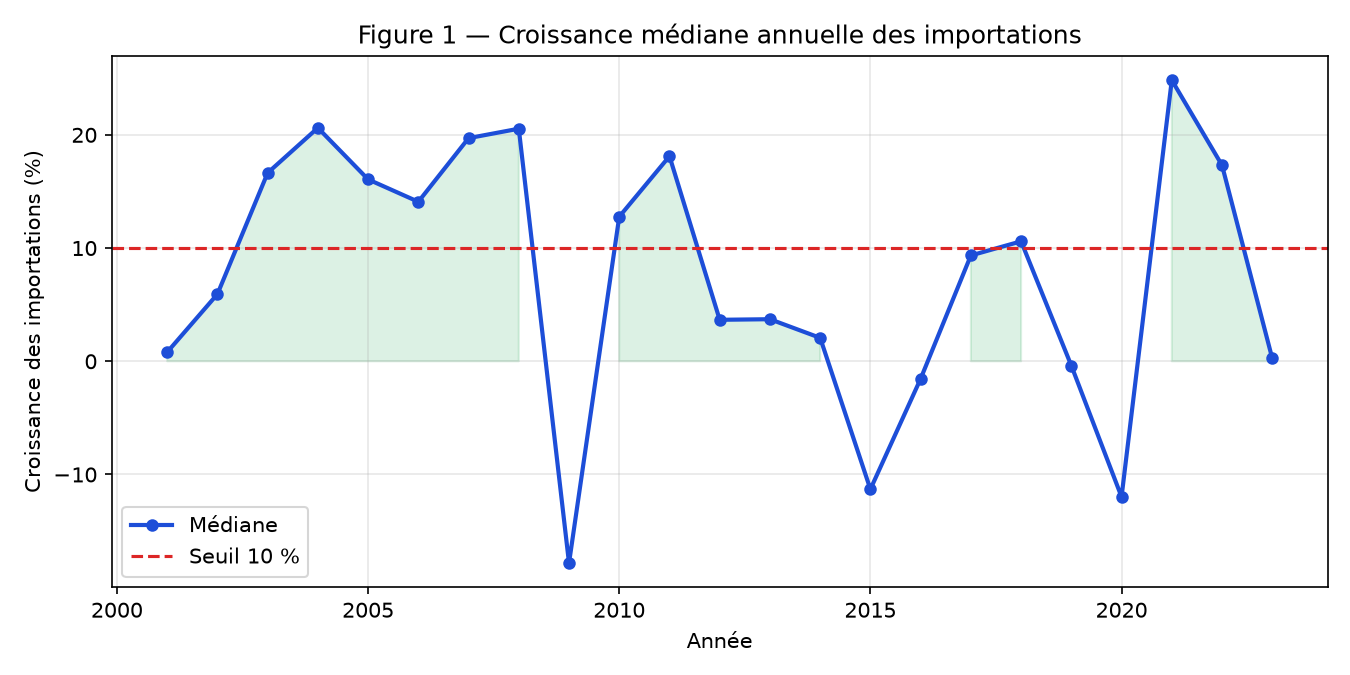
\includegraphics[width=\textwidth]{fig1_croissance_annuelle.png}
\par Croissance médiane : creux en 2009, 2015, 2020 ; rebond en 2021.
\column{0.45\textwidth}
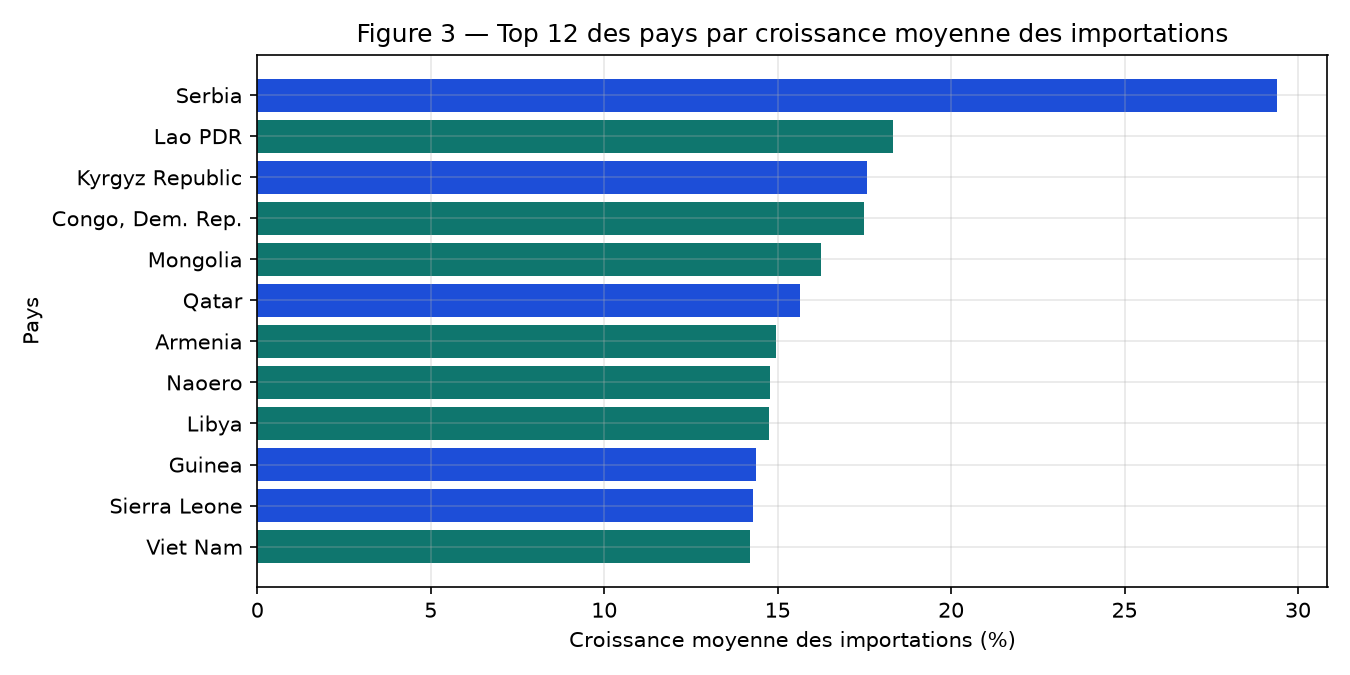
\includegraphics[width=\textwidth]{fig3_top_pays.png}
\par Pays les plus dynamiques : Serbie, Lao PDR, Kirghizistan.
\end{columns}
\end{frame}

\begin{frame}{4. Algorithme et protocole}
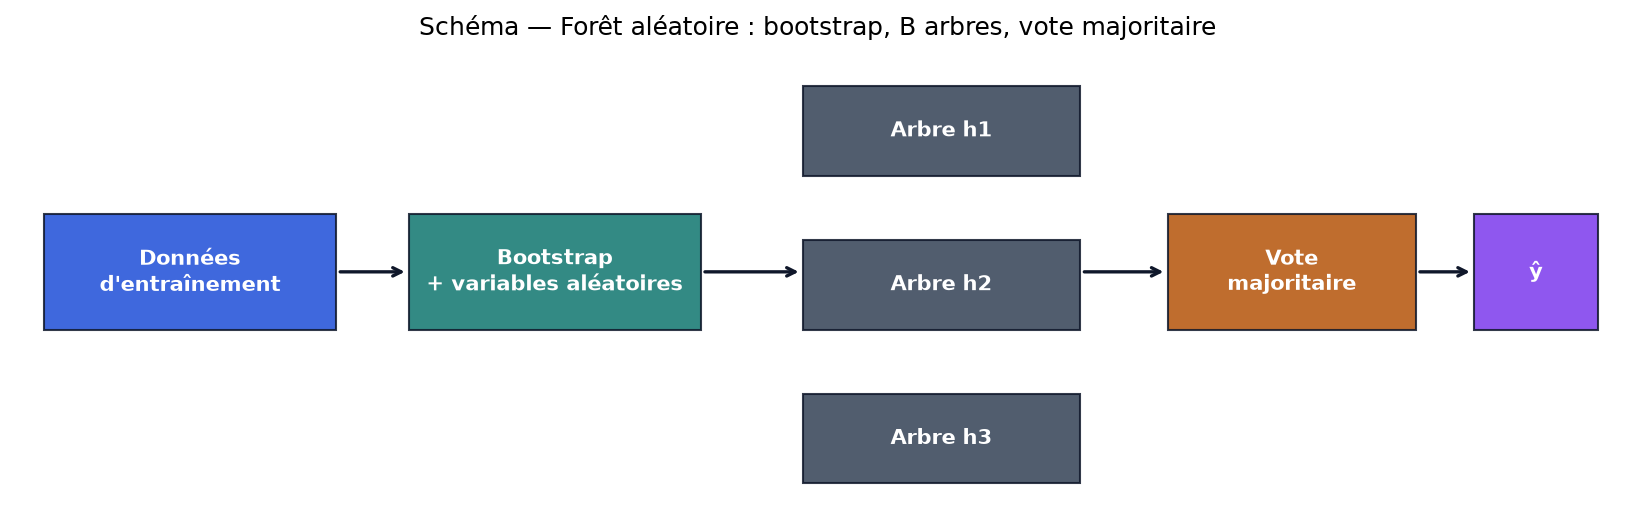
\includegraphics[width=0.92\textwidth]{schema_algorithme.png}
\par\textbf{Random Forest} (200 arbres) : bootstrap, sélection aléatoire de variables, vote majoritaire.
\par\textbf{Sans fuite :} variables passées uniquement ; entraînement $\leq$ 2019, test 2020--2023 ;
imputation/standardisation ajustées sur le train ; réglage par validation croisée stratifiée (5 plis).
\par Hyperparamètres : profondeur et minimum par feuille.
\end{frame}

\begin{frame}{5. Résultats}
\begin{tabular}{lccc}
\toprule
Méthode & F1 validation & F1 test & Accuracy test \\
\midrule
Référence naïve & 0.0 & 0.0 & 0.5 \\
Forêt aléatoire & 0.545 & 0.449 & 0.523 \\
\bottomrule
\end{tabular}
\par\bigskip
Précision 0.531, rappel 0.389, ROC-AUC 0.561. Matrice de confusion : {{233, 122}, {217, 138}}.
\par\bigskip
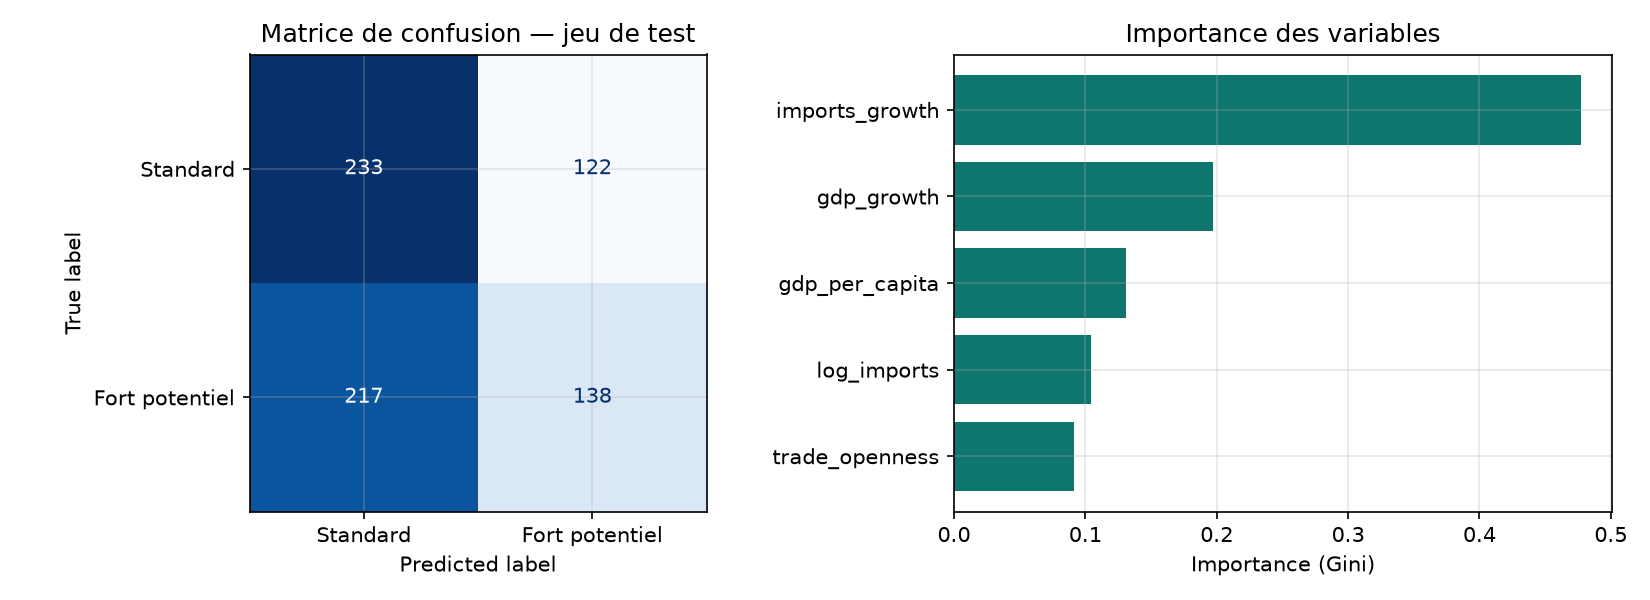
\includegraphics[width=0.8\textwidth]{fig4_resultats.png}
\end{frame}

\begin{frame}{6. Conclusion, limites, amélioration}
\textbf{Objectif ATTEINT :} F1 de 0.449 contre 0.0 pour la référence.
Le modèle aide à \textbf{présélectionner} des marchés, sans pronostic certain.
\par\bigskip
\textbf{Limites :} croissance annuelle volatile et faible corrélation passé/futur (r $\approx 0{,}11$) ;
données agrégées (pas de code SH) ; chocs 2020--2023.
\par\bigskip
\textbf{Amélioration :} flux bilatéraux par produit, horizon 3 ans, gradient boosting et
seuil de décision calibré selon le coût des erreurs.
\end{frame}
\end{document}
